\documentclass[a4paper,12pt]{extarticle}
\usepackage[utf8x]{inputenc}
\usepackage[T1,T2A]{fontenc}
\usepackage[russian]{babel}
\usepackage{hyperref}
\usepackage{indentfirst}
\usepackage{listings}
\usepackage{color}
\usepackage{xcolor}
\usepackage{here}
\usepackage{array}
\usepackage{multirow}
\usepackage{graphicx}
\usepackage{amsmath}

\hypersetup{
    colorlinks = false,
    linkbordercolor = {white}
}

\definecolor{string}{HTML}{B40000} % цвет строк в коде
\definecolor{comment}{HTML}{008000} % цвет комментариев в коде
\definecolor{keyword}{HTML}{1A00FF} % цвет ключевых слов в коде
\definecolor{morecomment}{HTML}{8000FF} % цвет include и других элементов в коде
\definecolor{сaptiontext}{HTML}{FFFFFF} % цвет текста заголовка в коде
\definecolor{сaptionbk}{HTML}{999999} % цвет фона заголовка в коде
\definecolor{bk}{HTML}{FFFFFF} % цвет фона в коде
\definecolor{frame}{HTML}{999999} % цвет рамки в коде
\definecolor{brackets}{HTML}{B40000} % цвет скобок в коде

\usepackage{caption}
\renewcommand{\lstlistingname}{Программа} % заголовок листингов кода

\bibliographystyle{ugost2008ls}

\usepackage{listings}
\lstset{ %
	extendedchars=\true,
	keepspaces=true,
	language=Python,						% choose the language of the code
	% Цвета
	keywordstyle=\color{keyword}\ttfamily\bfseries,
	%stringstyle=\color{string}\ttfamily,
	stringstyle=\ttfamily\color{red!50!brown},
	commentstyle=\color{comment}\ttfamily\itshape,
	morecomment=[l][\color{morecomment}]{\#},
	basicstyle=\footnotesize,		% the size of the fonts that are used for the code
	numbers=left,					% where to put the line-numbers
	numberstyle=\footnotesize,		% the size of the fonts that are used for the line-numbers
	stepnumber=1,					% the step between two line-numbers. If it is 1 each line will be numbered
	numbersep=5pt,					% how far the line-numbers are from the code
	backgroundcolor=\color{white},	% choose the background color. You must add \usepackage{color}
	showspaces=false				% show spaces adding particular underscores
	keywordstyle=color{blue}\bfseries, 
	showstringspaces=false,			% underline spaces within strings
	showtabs=false,					% show tabs within strings adding particular underscores
	frame=single,          		% adds a frame around the code
	tabsize=2,						% sets default tabsize to 2 spaces
	captionpos=t,					% sets the caption-position to top
	breaklines=true,				% sets automatic line breaking
	breakatwhitespace=false,		% sets if automatic breaks should only happen at whitespace
	escapeinside={\%*}{*)},			% if you want to add a comment within your code
	postbreak=\raisebox{0ex}[0ex][0ex]{\ensuremath{\color{red}\hookrightarrow\space}},
	texcl=true,
	inputpath=listings,                     % директория с листингами
}

\usepackage[left=2cm,right=2cm,
top=2cm,bottom=2cm,bindingoffset=0cm]{geometry}

%% Нумерация картинок по секциям
\usepackage{chngcntr}
\counterwithin{figure}{section}
\counterwithin{table}{section}

%%Точки нумерации заголовков
\usepackage{titlesec}
\titlelabel{\thetitle.\quad}
\usepackage[dotinlabels]{titletoc}

%% Оформления подписи рисунка
\addto\captionsrussian{\renewcommand{\figurename}{Рисунок}}
\captionsetup[figure]{labelsep = period}

%% Подпись таблицы
\DeclareCaptionFormat{hfillstart}{\hfill#1#2#3\par}
\captionsetup[table]{format=hfillstart,labelsep=newline,justification=centering,skip=-10pt,textfont=bf}

%% Путь к каталогу с рисунками
\graphicspath{{fig/}}

\begin{document}	% начало документа

% Титульная страница
%\begin{titlepage}	% начало титульной страницы

	\begin{center}		% выравнивание по центру

		Санкт-Петербургский Национально Исследовательский Университет\\
		информационных технологий, механики и оптики \\
		Кафедра систем управления и информатики\\[3cm]
		% название института, затем отступ 6см
		
		\huge \textbf{РЕФЕРАТ}\\[0.5cm]
		\large Электромеханические системы\\[0.1cm]
		\large Система автоматического управления квадракоптера Parrot ARDrone 2.0\\[2cm]

	\end{center}


	\begin{flushright} % выравнивание по правому краю
%		\begin{minipage}{0.5\textwidth} % врезка в половину ширины текста
%			\begin{flushleft} % выровнять её содержимое по левому краю

				\large Выполнили студенты группы P3335\\
				\large А.М. Зенкин\\[0.5cm]
				\large К.В. Карпов\\[0.5cm]
				
				\large Принял  к.т.н., доцент кафедры СУиР\\
				\sign[4cm]\large  М.С. Чежин\\
				\large Оценка: \sign\\
				«\underline{\hspace{0.7cm}}» \underline{\hspace{2cm}} \the\year г.

%			\end{flushleft}
%		\end{minipage}
	\end{flushright}
	
	\vfill % заполнить всё доступное ниже пространство

	\begin{center}
	\large Санкт-Петербург\\
	\large \the\year % вывести дату
	\end{center} % закончить выравнивание по центру

\thispagestyle{empty} % не нумеровать страницу
%\end{titlepage} % конец титульной страницы
\newpage


% Содержание
% Содержание
\renewcommand\contentsname{\centerline{Содержание}}
\tableofcontents
\thispagestyle{fancy}
\newpage





\section{Цель работы}
Изучить методику расчета режима резания аналитическим способом. Ознакомиться и приобрести навыки работы со справочной литературой.

\section{Варианты параметров}			
Заготовка, материал и его свойства: Отливка с коркой. Серый чугун СЧ $20 HB160;$\\

Вид обработки и параметр шероховатости: Обтачивание на проход $Ra = 12,5$ мкм;\\

$D = 120 mm;$\\

$d = 110h12;$\\

$l = 310 mm;$\\									
\section{Ход выполнения работы}

\subsection{Описание:}
На токарно-винторезном станке 16К20 производится черновое обтачивание на проход вала $D = 120$ мм до $d = 110h12$ мм. Длина обрабатываемой поверхности 310 мм; длина вала $l_1= 430$ мм. Заготовка - серый чугун 20 СЧ с пределом прочности $\sigma_b = 200$ МПа. Способ крепления заготовки - в центрах и поводковом патроне. Система СПИД недостаточно жесткая. Параметр шероховатости поверхности $Ra = 12,5$ мкм. Необходимо: выбрать режущий инструмент, назначить режим резания; определить основное время.

\subsection{Выполнение эскиза обработки:}
\begin{figure}[H]
	\begin{center}
		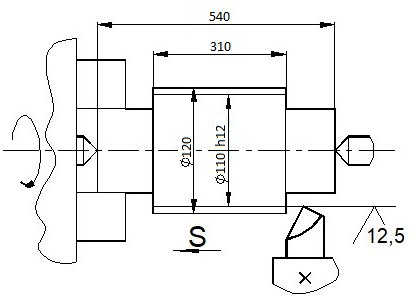
\includegraphics[scale=0.7]{1}
		\caption{Эскиз обработки} 
		\label{pic:pic_1} % название для ссылок внутри кода
	\end{center}
\end{figure}

\subsection{Выбор режущего инструмента:}
Для обтачивания на проход вала из стали 40Х принимаем токарный проходной резец прямой правый с пластинкой из твердого сплава ВК6. Форма передней поверхности радиусная с фаской; геометрические параметры режущей части резца:\\
$\gamma=15^{\circ}$; $\alpha=12^{\circ}$; $\lambda=0$,\\ 
$\phi=60^{\circ}$ ; $\phi_1=30^{\circ}$,\\
$r=1$ мм; $f=1$ мм.

\subsection{Назначение глубины резания:}
Глубина резания. При черновой обработке припуск срезаем за один проход, тогда:\\
\begin{equation}
	\begin{split}
		&t=h=\dfrac{D-d}{2}=\dfrac{120-110}{2} = 5 mm;
	\end{split}
\end{equation}

\subsection{Определение подачи:}
Назначаем подачу. Для черновой обработки заготовки из серого чегуна диаметром до 400 мм резцом сечения $16$x$25$ при глубине резания до 5мм. $S=0,9$ мм/об.

\subsection{Рассчёт скорости резания:}
Скорость резания , допускаемая материалом резца:
\begin{equation}
	\begin{split}
		&V=\dfrac{C_v}{T^mt^xS^y}K_v, m/min\\
		&C_v=243, x=0.15, y=0.4, m=0.2, T=60 min\\
	\end{split}
\end{equation}
Поправочный коэффициент для обработки резцом с твердосплавной пластиной:
\begin{equation}
	\begin{split}
		&K_v = K_{mv}\cdot K_{nv}\cdot K_{uv}\cdot K_{\phi v};\\
		&K_{mv} = \left( \dfrac{190}{\sigma_b} \right)^{n_v}, n_v = 1;\\
		&K_{nv}=0.8, \\
		&K_{uv}=0.83, \\
		&K_{\phi v}=0.9; \\
		&V = \dfrac{243}{60^{0.2}\cdot 5^{0.15}\cdot 0.9^{0.4}}\cdot 1.34 \cdot 0.83\cdot 0.8\cdot 0.9 = 73.65 m/min
	\end{split}
\end{equation}

\newpage

\subsection{Определение частоты вращения шпинделя и корректирование по паспорту станка:}
Частота вращения, соответствующая найденной скорости резания:
\begin{equation}
	\begin{split}
		&n=\dfrac{1000V}{\pi \cdot D}, rpm;\\
		&n=\dfrac{1000\cdot 73.65}{3.14\cdot 120}=195.47 rpm;\\
	\end{split}
\end{equation}

Корректируем частоту вращения шпинделя по паспортным данным станка:
\begin{equation}
	\begin{split}
		&n_d = 200 rpm;\\
	\end{split}
\end{equation}

\subsection{Определение действительной скорости резания:}
Действительная скорость резания:
\begin{equation}
	\begin{split}
		&V_d = \dfrac{\pi\cdot D\cdot n}{1000}, m/min;\\
		&V_d = \dfrac{3.14\cdot 120\cdot 200}{1000} =75.36 m/min;
	\end{split}
\end{equation}

\subsection{Рассчёт основного технологического времени:}
Основное время:
\begin{equation}
	\begin{split}
		&T_o = \dfrac{L}{n\cdot S}\cdot i, min;
	\end{split}
\end{equation}
Путь резца: $L=1+y+\delta$,  мм;\\
Врезание резца: $y=t\cdot ctg(\phi) = 5\cdot ctg(60^{\circ}) = 5\cdot 0.58 = 2.9$ мм;\\
Пробег резца: $\delta = 2.5$ мм;\\
Тогда: $L=310 + 2.5 + 2.9 = 315.4$ мм;\\
\begin{equation}
	\begin{split}
		&T_o = \dfrac{315.4}{200\cdot 0.9}\cdot = 1.75 min;
	\end{split}
\end{equation}

\section{Вывод}
В данной лабораторной работе была изучена методика расчёта режима резания аналитическим способом, а также были приобретены навыки работы со справочной литературой. Был построен эскиз обработки (рис. \ref{pic:pic_1}).
\end{document}
